\documentclass[a4paper,8pt,twocolumn]{article}
\usepackage[UTF8]{ctex}
\usepackage{graphicx}
\usepackage{fancyhdr}
\usepackage{amsmath}
\usepackage{subcaption}
\usepackage{float}
\usepackage[
  left=2cm,
  right=2cm,
  top=1.5cm,
  bottom=2.5cm
]{geometry}
\usepackage{siunitx}
\usepackage{booktabs}
\usepackage{enumitem}
\usepackage{array}
\usepackage{tabularx}
\newcolumntype{Y}{>{\centering\arraybackslash}X}
\usepackage{amssymb}
\usepackage{pgfplots}
\usepackage{pgfplotstable}
\pgfplotsset{compat=1.18}

%================ 温度-时间曲线统一样式 ================
\pgfplotsset{
  tempplot/.style={
    width=0.9\columnwidth,
    height=0.20\textheight,
    scale only axis,
    grid=major,
    enlargelimits=false,
    xlabel={时间 $\tau$ / s},
    ylabel={温度 / \si{\degreeCelsius}},
    title style={font=\small},
    label style={font=\small},
    ticklabel style={font=\scriptsize},
    legend style={font=\scriptsize, at={(0.02,0.98)}, anchor=north west,
                  cells={anchor=west}}
  }
}
%=======================================================

\sisetup{
  per-mode=symbol,
  separate-uncertainty = true
}

\title{
  \textbf{\huge RX1：热传导过程的COMSOL模拟}
}
\author{
  黄雨~24352027\\
  \small 中山大学物理学院~广东~广州
}

\pagestyle{fancy}
\fancyhf{}
\fancyhead[C]{RX1：热传导过程的COMSOL模拟}
\fancyfoot[C]{\thepage}

\begin{document}
\maketitle
\newpage

%%%%%%%%%%%%%%%%%%%%%%%%%%%%%%%%%%%%%%%%%%%%%%%%%%%%%%%%%%%%
\section{实验目的}

\begin{enumerate}
  \item 了解采用COMSOL进行有限元分析的方法；
  \item 利用COMSOL模拟不良热导体的热传导过程；
  \item 通过评估模拟结果与实验结果的异同，研究影响热传导的宏观参数。
\end{enumerate}

%%%%%%%%%%%%%%%%%%%%%%%%%%%%%%%%%%%%%%%%%%%%%%%%%%%%%%%%%%%%
\section{实验仪器与装置}

\begin{itemize}
  \item 实验测控用计算机（已安装COMSOL Multiphysics及LabVIEW软件）。
\end{itemize}

%%%%%%%%%%%%%%%%%%%%%%%%%%%%%%%%%%%%%%%%%%%%%%%%%%%%%%%%%%%%
\section{实验原理}

本实验利用COMSOL软件模拟不良热导体实验中的加热过程，以得到温差及中心面温度随时间的变化关系。

考虑如图\,1\,所示的一维无限大导热模型：一无限大不良热导体平板，厚度为$2R$，初始温度均匀为$t_0$，在平板两侧同时施加均匀的、指向中心面的热流密度$q_c$。以样品中心为坐标原点，热运动方程组为
\begin{equation}
  \left\{
    \begin{aligned}
      &\frac{\partial t(x,\tau)}{\partial \tau}
        = a\,\frac{\partial^2 t(x,\tau)}{\partial x^2}\\[4pt]
      &\frac{\partial t(R,\tau)}{\partial x}=\frac{q_c}{\lambda},
        \quad\frac{\partial t(0,\tau)}{\partial x}=0\\[4pt]
      &t(x,0)=t_0
    \end{aligned}
  \right.
  \tag{RX1.1}
\end{equation}
其中$a=\lambda/\rho c$为热扩散率，$q_c=c\rho R\,\partial t/\partial\tau$，$\lambda$为导热系数，$\rho$为密度，$c$为比热容。

方程（RX1.1）的精确解为
\begin{equation}
  \begin{split}
    t(x,\tau) &= t_0 + \frac{q_c}{\lambda}
    \Bigg[\frac{a\tau}{R}+\frac{x^2}{2R}-\frac{R}{6}\\
    &\quad +\frac{2R}{\pi^2}\sum_{n=1}^{\infty}
      \frac{(-1)^{n+1}}{n^2}\cos\!\frac{n\pi x}{R}
      \cdot e^{-\frac{an^2\pi^2}{R^2}\tau}\Bigg]
  \end{split}
  \tag{RX1.2}
\end{equation}

当加热时间$\tau$满足$a\tau/R^2>0.5$时，式（RX1.2）中的级数求和项因指数衰减可以忽略，公式简化为
\begin{equation}
  t(x,\tau)=t_0+\frac{q_c}{\lambda}
  \!\left[\frac{a\tau}{R}+\frac{x^2}{2R}-\frac{R}{6}\right]
  \tag{RX1.3}
\end{equation}

由此得到样品中心面（$x=0$）和加热面（$x=R$）的温度分别为
\begin{equation}
  \begin{cases}
    \displaystyle t(0,\tau)=t_0+\frac{q_c}{\lambda}
      \!\left[\frac{a\tau}{R}-\frac{R}{6}\right]\\[8pt]
    \displaystyle t(R,\tau)=t_0+\frac{q_c}{\lambda}
      \!\left[\frac{a\tau}{R}+\frac{R}{3}\right]
  \end{cases}
  \tag{RX1.4}
\end{equation}

两处温度均以速率$aq_c/\lambda R$线性上升，而加热面与中心面之间的温度差
\begin{equation}
  \Delta t = t(R,\tau)-t(0,\tau)=\frac{q_c R}{2\lambda}
  \tag{RX1.5}
\end{equation}
与加热时间$\tau$无关，保持恒定——此状态称为\textbf{准稳态}。

由式（RX1.5）可得样品热传导率
\begin{equation}
  \lambda=\frac{q_c R}{2\Delta t}
  \tag{RX1.6}
\end{equation}
以及样品比热容
\begin{equation}
  c=\frac{q_c}{\rho R\,\mathrm{d}t/\mathrm{d}\tau}
  \tag{RX1.7}
\end{equation}
其中$\mathrm{d}t/\mathrm{d}\tau$为准稳态下样品各处相同的升温速率。

%%%%%%%%%%%%%%%%%%%%%%%%%%%%%%%%%%%%%%%%%%%%%%%%%%%%%%%%%%%%
\section{实验内容与步骤}

\subsection{双平板样品升温模型的建立}

有限元分析一般包括前处理（几何建模、定义材料、网格划分、设置边界条件与分析类型）、求解（方程建立与计算）和后处理（物理量计算、可视化、数据导出）三个阶段。本部分以双平板样品为对象，详细介绍具体操作：

\begin{enumerate}[label=(\arabic*)]
  \item 运行COMSOL Multiphysics，通过"模型向导"构建平板样品加热模型。
  \item 在"选择空间维度"界面选"三维"。
  \item 选择物理场：\textbf{传热\,$\to$\,固体传热（ht）}，单击"添加"后进入"研究"。
  \item 选择研究类型：\textbf{预设研究\,$\to$\,瞬态}，单击"完成"进入主界面。
  \item 设置全局参数：添加\texttt{Volt}（加热电压）、\texttt{Rr}（加热膜电阻）、\texttt{AA}（修正因子）、\texttt{Qc}（发热功率）、\texttt{SS}（横截面积）、\texttt{qin}（单侧热流密度）共六个参数，并填入表达式与数值。注意COMSOL对大小写敏感。
  \item 构建几何体：依次添加两个长方体，尺寸均为宽度\,$\SI{10}{mm}$\,、深度\,$\SI{90}{mm}$\,、高度\,$\SI{90}{mm}$；第一块坐标原点位于$(0,0,0)$，第二块位于$(10,0,0)$\,mm；选"形成联合体"后"全部构建"，完成由"2个域、11个边界、20条边及12个顶点"组成的联合体。
  \item 选择材料：右击"材料"\,$\to$\,"空材料"，填入有机玻璃（或橡胶）参数——导热系数$\lambda=\SI{0.168}{W/(m\cdot K)}$、密度$\rho=\SI{1196}{kg/m^3}$、恒压热容$C_p=\SI{1333}{J/(kg\cdot K)}$，并保存为用户定义材料备用。
  \item 设置固体传热模型：
    \begin{itemize}
      \item \textbf{热通量}：选定联合体前后两面，设置广义向内热流密度为全局变量\texttt{qin}（对应边界编号1和11）；
      \item \textbf{热绝缘}：选定联合体周围四个侧面（边界编号4、5、9），施加绝热边界条件。
    \end{itemize}
  \item 设置域点探针：
    \begin{itemize}
      \item 中心面探针：坐标$(10,\,4.5,\,4.5)$\,mm；
      \item 加热面探针：坐标$(20,\,4.5,\,4.5)$\,mm。
    \end{itemize}
  \item 设置网格：单元尺寸选"细化"，单击"全部构建"生成网格。
  \item 设置研究参数：时间\texttt{range(1,30,600)}（即$0$至$\SI{600}{s}$，每隔$\SI{30}{s}$保存一次），点击"$=$\,计算"开始求解。
  \item 后处理：在"结果"中查看温度云图及探针时序曲线，导出中心面与加热面温度数据，计算约10分钟时的温度差$\Delta T$和升温速率$\mathrm{d}T/\mathrm{d}t$，与上学期实验结果对比，评价模拟与实验的异同。
\end{enumerate}

\subsection{四样品的模拟}

在双平板模型基础上，构建更接近实际实验的仿真模型：四块有机玻璃（或橡胶）样品板加两块加热膜（加热膜厚度$l=\SI{0.123}{mm}$），共六个长方体。前后两个加热面和六块板四周侧面均设为绝热。两块加热膜均以修正功率$Q_p$加热（全局参数保持不变）。网格划分时，对两块加热膜选"细化"，其余四块样品板选常规网格。

\subsection{四样品且无修正因子$A$的模拟（一）}

取$A=1$（不使用修正因子），在六块板（含加热膜）四周增加PP阻热层，阻热层与外界空气之间满足\textbf{第三类边界条件}（对流换热），热交换系数取$h=\SI{150}{W/(m^2\cdot K)}$（可适当调整）。六块板前后仅与样品接触的板面设为绝热，其余边界满足对流换热条件。阻热层尺寸：底部高$\SI{45}{mm}$，左右边宽各$\SI{63}{mm}$，顶部高$\SI{40}{mm}$，总厚度约$\SI{40.246}{mm}$（材料参数参照PP板实际数据）。注意加热膜主体为聚酰亚胺薄膜（约占体积的5/6），通电加热片（铝箔，厚度$\SI{0.03}{mm}$，约占体积的1/6）嵌于薄膜正中。

\subsection{四样品且无修正因子$A$的模拟（二）}

在模拟（一）基础上进一步完善，使模型严格对应实际实验装置：

\begin{itemize}
  \item \textbf{阻热层（PP板）}：$\lambda=\SI{0.90}{W/(m\cdot K)}$，$c_p=\SI{1900}{J/(kg\cdot K)}$，$\rho=\SI{920}{kg/m^3}$，尺寸与模拟（一）相同；
  \item \textbf{前后隔热泡沫板}（不完全绝热）：$\lambda=\SI{0.046}{W/(m\cdot K)}$，$c_p=\SI{4200}{J/(kg\cdot K)}$，$\rho=\SI{400}{kg/m^3}$，截面为$\SI{122}{mm}\times\SI{122}{mm}$正方形，厚度$\SI{47}{mm}$（左右对称），周围固定泡沫的木板框厚度$\SI{5}{mm}$（可忽略）；
  \item \textbf{加热膜}改用嵌铜箔面膜：$\lambda=\SI{67.09}{W/(m\cdot K)}$，$\rho=\SI{1681.1}{kg/m^3}$，$c_p=\SI{1090}{J/(kg\cdot K)}$；
  \item 阻热层及泡沫板外表面均以$h=\SI{150}{W/(m^2\cdot K)}$与周围空气交换热量，满足第三类边界条件。
\end{itemize}

\subsection{修正因子$A$的确定}

回到两块样品（双平板）情形，通过逐步调整热流密度修正因子$A$并重复运行COMSOL模拟，确定当$A$取何值时仿真结果与实际实验测量值相符。具体计算方法和结果见§\,\ref{sec:results}。

%%%%%%%%%%%%%%%%%%%%%%%%%%%%%%%%%%%%%%%%%%%%%%%%%%%%%%%%%%%%

\section{实验结果与分析}
\label{sec:results}

\subsection{实验测量原始数据}

实验采用两块厚度$R=\SI{10}{mm}$的样品，热电偶夹持于两板中间（中心面），另一热电偶置于加热面，分别在$\SI{16}{V}$与$\SI{19}{V}$两种加热电压下记录温度随时间的变化。

\begin{figure}[htbp]
  \centering
  \begin{tikzpicture}
  \begin{axis}[
      tempplot,
      title={有机玻璃温度随时间变化},
      legend entries={16V 中心面, 16V 加热面, 19V 中心面, 19V 加热面}
  ]
    \addplot[mark=none,blue,thick] coordinates {
      (0,1.0)(30,1.0)(60,1.1)(90,1.3)(120,1.5)(150,1.5)(180,1.5)(210,1.5)
      (240,1.5)(270,1.5)(300,1.5)(330,1.5)(360,1.5)(390,1.5)(420,1.5)
      (450,1.5)(480,1.5)(510,1.5)(540,1.5)(570,1.5)(600,1.5)(630,1.5)
      (660,1.6)(690,1.6)(720,1.6)(750,1.6)(780,1.6)(810,1.6)(840,1.6)
      (870,1.6)(900,1.6)};
    \addplot[mark=none,blue,thick,dashed] coordinates {
      (0,0.5)(30,0.5)(60,0.6)(90,0.6)(120,0.8)(150,1.0)(180,1.3)(210,1.5)
      (240,1.7)(270,2.0)(300,2.3)(330,2.7)(360,2.8)(390,2.9)(420,3.1)
      (450,3.2)(480,3.3)(510,3.5)(540,3.8)(570,4.0)(600,4.2)(630,4.5)
      (660,4.8)(690,5.0)(720,5.0)(750,5.0)(780,5.5)(810,5.9)(840,6.1)
      (870,6.2)(900,6.2)};
    \addplot[mark=none,red,thick] coordinates {
      (0,1.0)(30,2.0)(60,2.9)(90,3.4)(120,3.8)(150,4.0)(180,4.2)(210,4.3)
      (240,4.5)(270,4.7)(300,4.8)(330,4.8)(360,4.9)(390,5.0)(420,5.0)
      (450,5.0)(480,5.1)(510,5.0)(540,5.0)(570,5.0)(600,5.0)(630,5.0)
      (660,5.0)(690,5.0)(720,5.0)(750,5.0)(780,5.0)(810,5.0)(840,5.0)
      (870,5.0)(900,5.1)};
    \addplot[mark=none,red,thick,dashed] coordinates {
      (0,4.9)(30,4.9)(60,4.9)(90,4.9)(120,5.0)(150,5.0)(180,5.2)(210,5.3)
      (240,5.7)(270,6.0)(300,6.4)(330,6.8)(360,7.0)(390,7.2)(420,7.6)
      (450,8.0)(480,8.2)(510,8.5)(540,8.9)(570,9.2)(600,9.5)(630,9.8)
      (660,10.0)(690,10.2)(720,10.6)(750,11.0)(780,11.2)(810,11.5)
      (840,11.7)(870,12.0)(900,12.0)};
  \end{axis}
  \end{tikzpicture}
  \caption{有机玻璃样品中心面与加热面温度随时间变化}
  \label{fig:acrylic}
\end{figure}

\begin{figure}[htbp]
  \centering
  \begin{tikzpicture}
  \begin{axis}[
      tempplot,
      title={橡胶温度随时间变化},
      legend entries={16V 中心面, 16V 加热面, 19V 中心面, 19V 加热面}
  ]
    \addplot[mark=none,blue,thick] coordinates {
      (0,1.0)(30,1.5)(60,2.0)(90,2.5)(120,3.0)(150,3.0)(180,3.0)(210,3.0)
      (240,3.1)(270,3.3)(300,3.5)(330,3.5)(360,3.5)(390,3.5)(420,3.5)
      (450,3.5)(480,3.5)(510,3.5)(540,3.5)(570,3.5)(600,3.5)(630,3.5)
      (660,3.6)(690,3.6)(720,3.6)(750,3.6)(780,3.6)(810,3.6)(840,3.6)
      (870,3.6)(900,3.6)};
    \addplot[mark=none,blue,thick,dashed] coordinates {
      (0,6.0)(30,6.0)(60,6.1)(90,6.2)(120,6.4)(150,6.5)(180,6.6)(210,6.7)
      (240,6.9)(270,7.0)(300,7.4)(330,7.8)(360,8.0)(390,8.2)(420,8.3)
      (450,8.4)(480,8.6)(510,8.7)(540,8.9)(570,9.1)(600,9.3)(630,9.5)
      (660,9.7)(690,10.0)(720,10.2)(750,10.5)(780,10.7)(810,11.0)
      (840,11.2)(870,11.5)(900,11.5)};
    \addplot[mark=none,red,thick] coordinates {
      (0,1.0)(30,1.3)(60,1.5)(90,1.8)(120,2.1)(150,2.1)(180,2.2)(210,2.2)
      (240,2.3)(270,2.3)(300,2.3)(330,2.4)(360,2.4)(390,2.4)(420,2.5)
      (450,2.5)(480,2.5)(510,2.5)(540,2.5)(570,2.5)(600,2.6)(630,2.6)
      (660,2.6)(690,2.6)(720,2.6)(750,2.6)(780,2.6)(810,2.6)(840,2.6)
      (870,2.6)(900,2.6)};
    \addplot[mark=none,red,thick,dashed] coordinates {
      (0,1.9)(30,1.9)(60,2.0)(90,2.1)(120,2.3)(150,2.6)(180,2.9)(210,3.2)
      (240,2.5)(270,3.8)(300,4.2)(330,4.5)(360,4.7)(390,5.0)(420,5.2)
      (450,5.4)(480,5.7)(510,6.1)(540,6.5)(570,6.8)(600,7.0)(630,7.2)
      (660,7.6)(690,8.0)(720,8.3)(750,8.5)(780,8.7)(810,9.0)(840,9.3)
      (870,9.5)(900,9.5)};
  \end{axis}
  \end{tikzpicture}
  \caption{橡胶样品中心面与加热面温度随时间变化（$t=\SI{240}{s}$处波动为测量噪声）}
  \label{fig:rubber}
\end{figure}

由图可见，加热约$\SI{150}{\second}$至$\SI{300}{\second}$后，中心面升温速率趋于平稳，加热面温度仍持续线性上升，温度差$\Delta T$在$\SI{900}{\second}$内尚未完全收敛，说明准稳态需超过$\SI{900}{\second}$后才能建立。取$t=\SI{900}{s}$末态数值作为近似准稳态参考值，列于表\,\ref{tab:exp_quasisteady}。

\begin{table}[H]
\centering
\caption{各工况末态（$t=\SI{900}{s}$）近似准稳态温度差}
\label{tab:exp_quasisteady}
\begin{tabular}{lccc}
\toprule
样品 & 电压 & $T_{\text{加热面}}$(\si{\degreeCelsius}) & $\Delta T$(\si{\degreeCelsius})\\
\midrule
有机玻璃 & 16 V & 6.2 & 4.6 \\
有机玻璃 & 19 V & 12.0 & 6.9 \\
橡胶     & 16 V & 11.5 & 7.9 \\
橡胶     & 19 V & 9.5  & 6.9 \\
\bottomrule
\end{tabular}
\end{table}

\subsection{模拟（一）结果及修正因子$A$的确定}

在六块板（四块样品板＋两块加热膜）四周加PP阻热层、前后两面热绝缘的简化模型中，先取$A=1$运行仿真，得准稳态温度差$\Delta T_{\text{sim1}}$；再逐步调整$A$至仿真结果与实验值吻合，求得修正因子。理论关系式为
\begin{equation}
  A = \frac{\Delta T_{\text{exp}}}{\Delta T_{\text{sim1}}(A=1)}.
  \tag{RX1.8}
\end{equation}

\begin{figure}[htbp]
  \centering
  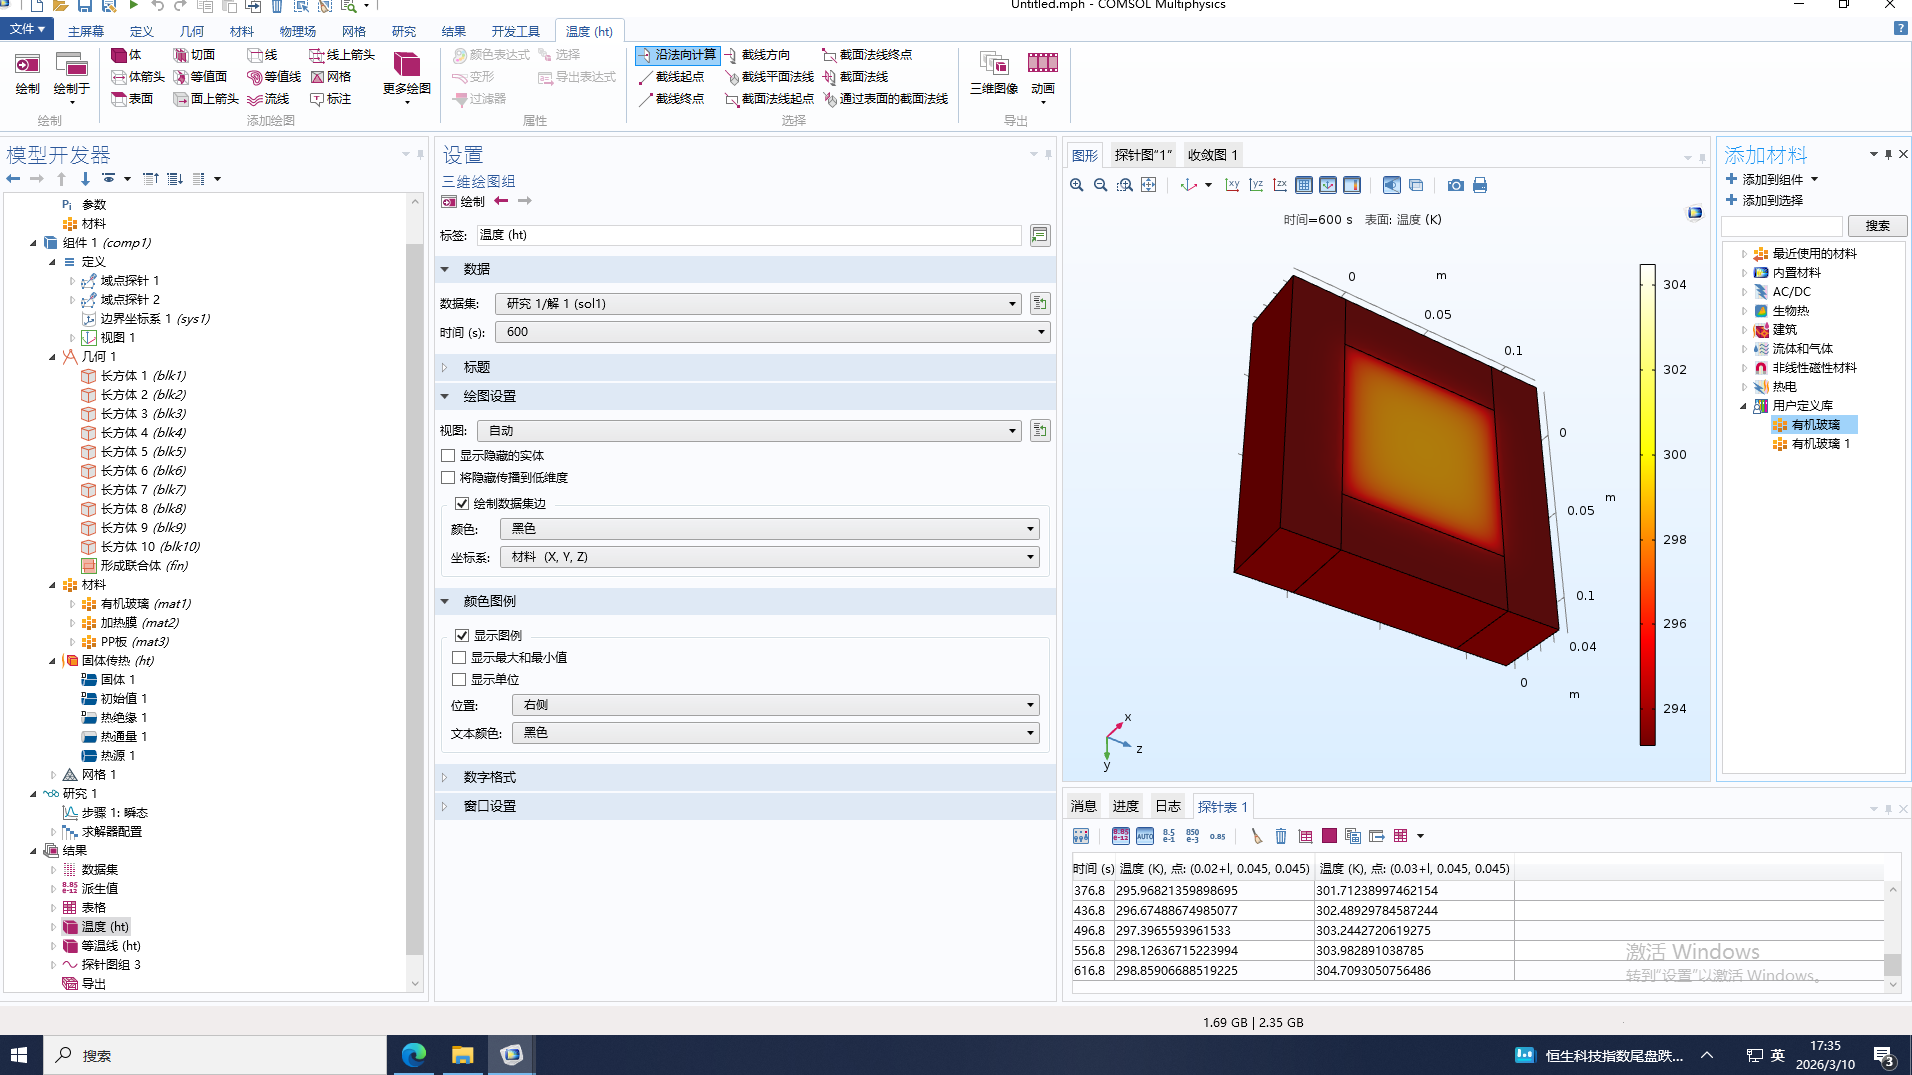
\includegraphics[width=0.95\columnwidth]{模拟一温度云图.png}
  \caption{模拟（一）温度分布云图（PP阻热层，$A=1$）}
\end{figure}

\begin{figure}[htbp]
  \centering
  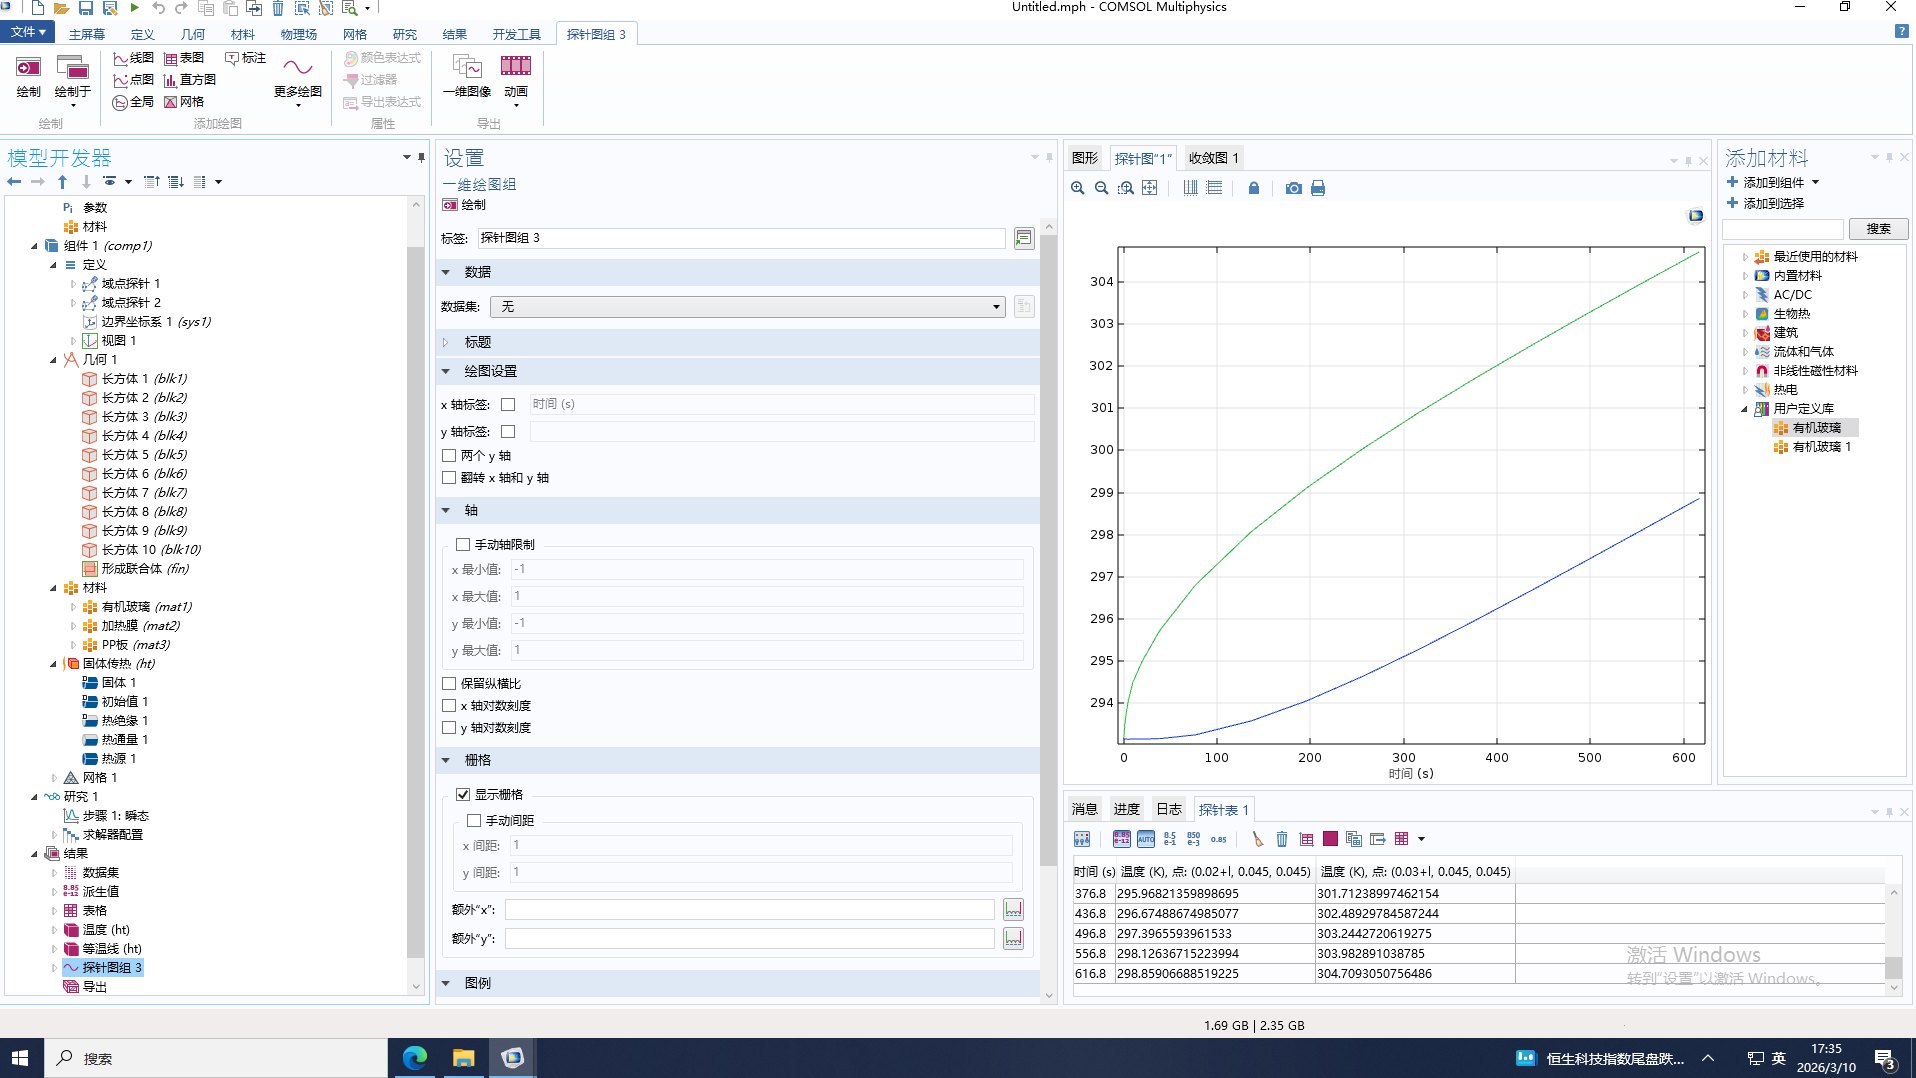
\includegraphics[width=0.95\columnwidth]{模拟一时序曲线.png}
  \caption{模拟（一）中心面与加热面温度随时间变化}
\end{figure}

取有机玻璃16\,V工况（$\Delta T_{\text{exp}}\approx\SI{4.6}{\degreeCelsius}$），将模拟（一）$A=1$时的准稳态$\Delta T_{\text{sim1}}$代入式（RX1.8）即可得修正因子$A$：

\begin{table}[H]
\centering
\caption{双平板修正因子$A$（有机玻璃16 V）}
\begin{tabular}{ccc}
\toprule
$\Delta T_{\text{exp}}$(\si{K}) & $\Delta T_{\text{sim1}}(A=1)$(\si{K}) & $A$ \\
\midrule
4.6 & \quad 4.13 \quad & 0.69 \\
\bottomrule
\end{tabular}
\end{table}

\subsection{模拟（二）结果（严格对应真实情况）}

在含PP阻热层及泡沫隔热板、嵌铜箔加热膜、$A=1$的完整模型（共12个长方体）中运行仿真，COMSOL导出的两探针温度时序数据如图\,\ref{fig:sim2}所示。

\begin{figure}[htbp]
  \centering
  \begin{tikzpicture}
  \begin{axis}[
      tempplot,
      title={模拟（二）两探针温度随时间变化},
      ylabel={温度 / K},
      legend entries={中心面探针, 加热面探针}
  ]
    \addplot[mark=*,mark size=1.5pt,blue,thick] coordinates {
      (753.6,300.25)(873.6,301.54)(993.6,302.78)
      (1113.6,303.97)(1233.6,305.11)};
    \addplot[mark=square*,mark size=1.5pt,green!60!black,thick] coordinates {
      (753.6,306.12)(873.6,307.40)(993.6,308.34)
      (1113.6,308.94)(1233.6,309.24)};
  \end{axis}
  \end{tikzpicture}
  \caption{模拟（二）COMSOL导出探针温度数据}
  \label{fig:sim2}
\end{figure}

\begin{figure}[htbp]
  \centering
  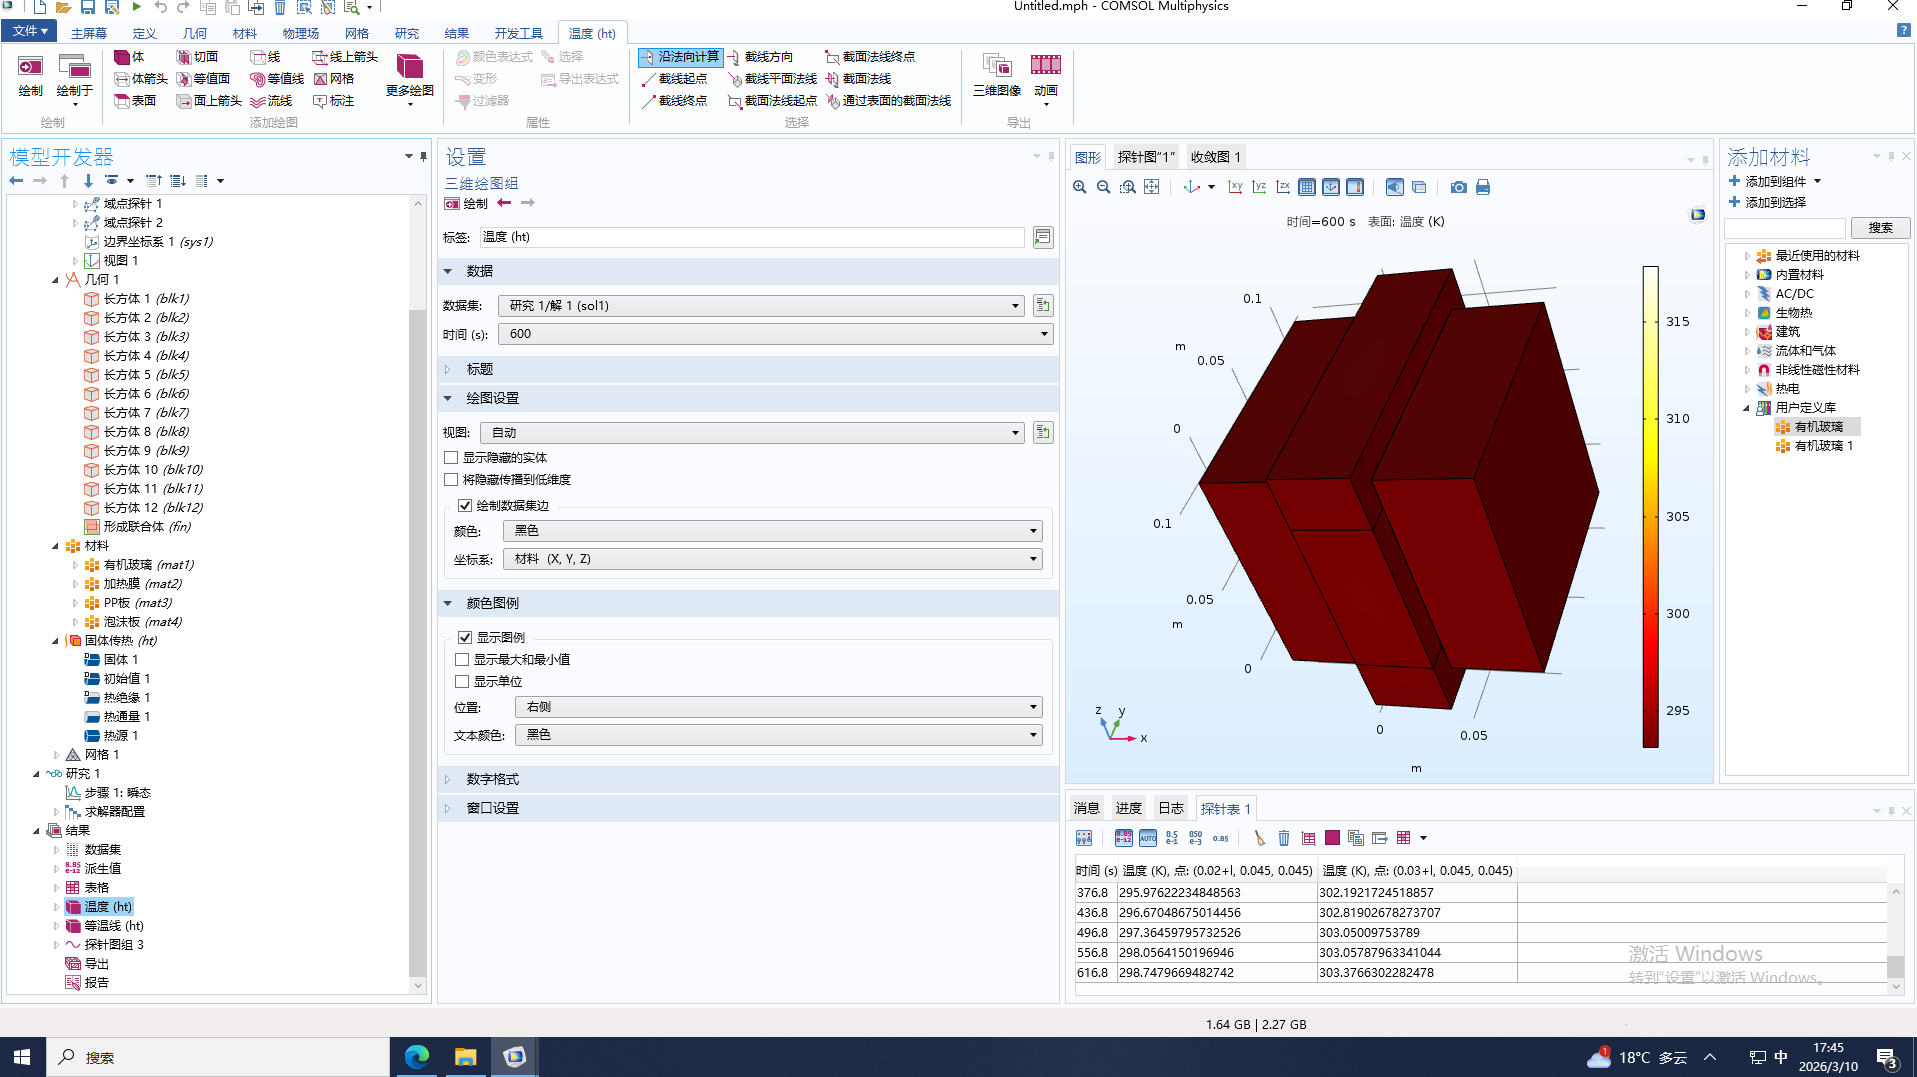
\includegraphics[width=0.95\columnwidth]{真实模拟温度云图.png}
  \caption{模拟（二）温度分布云图（完整模型，$A=1$）}
\end{figure}

\begin{figure}[htbp]
  \centering
  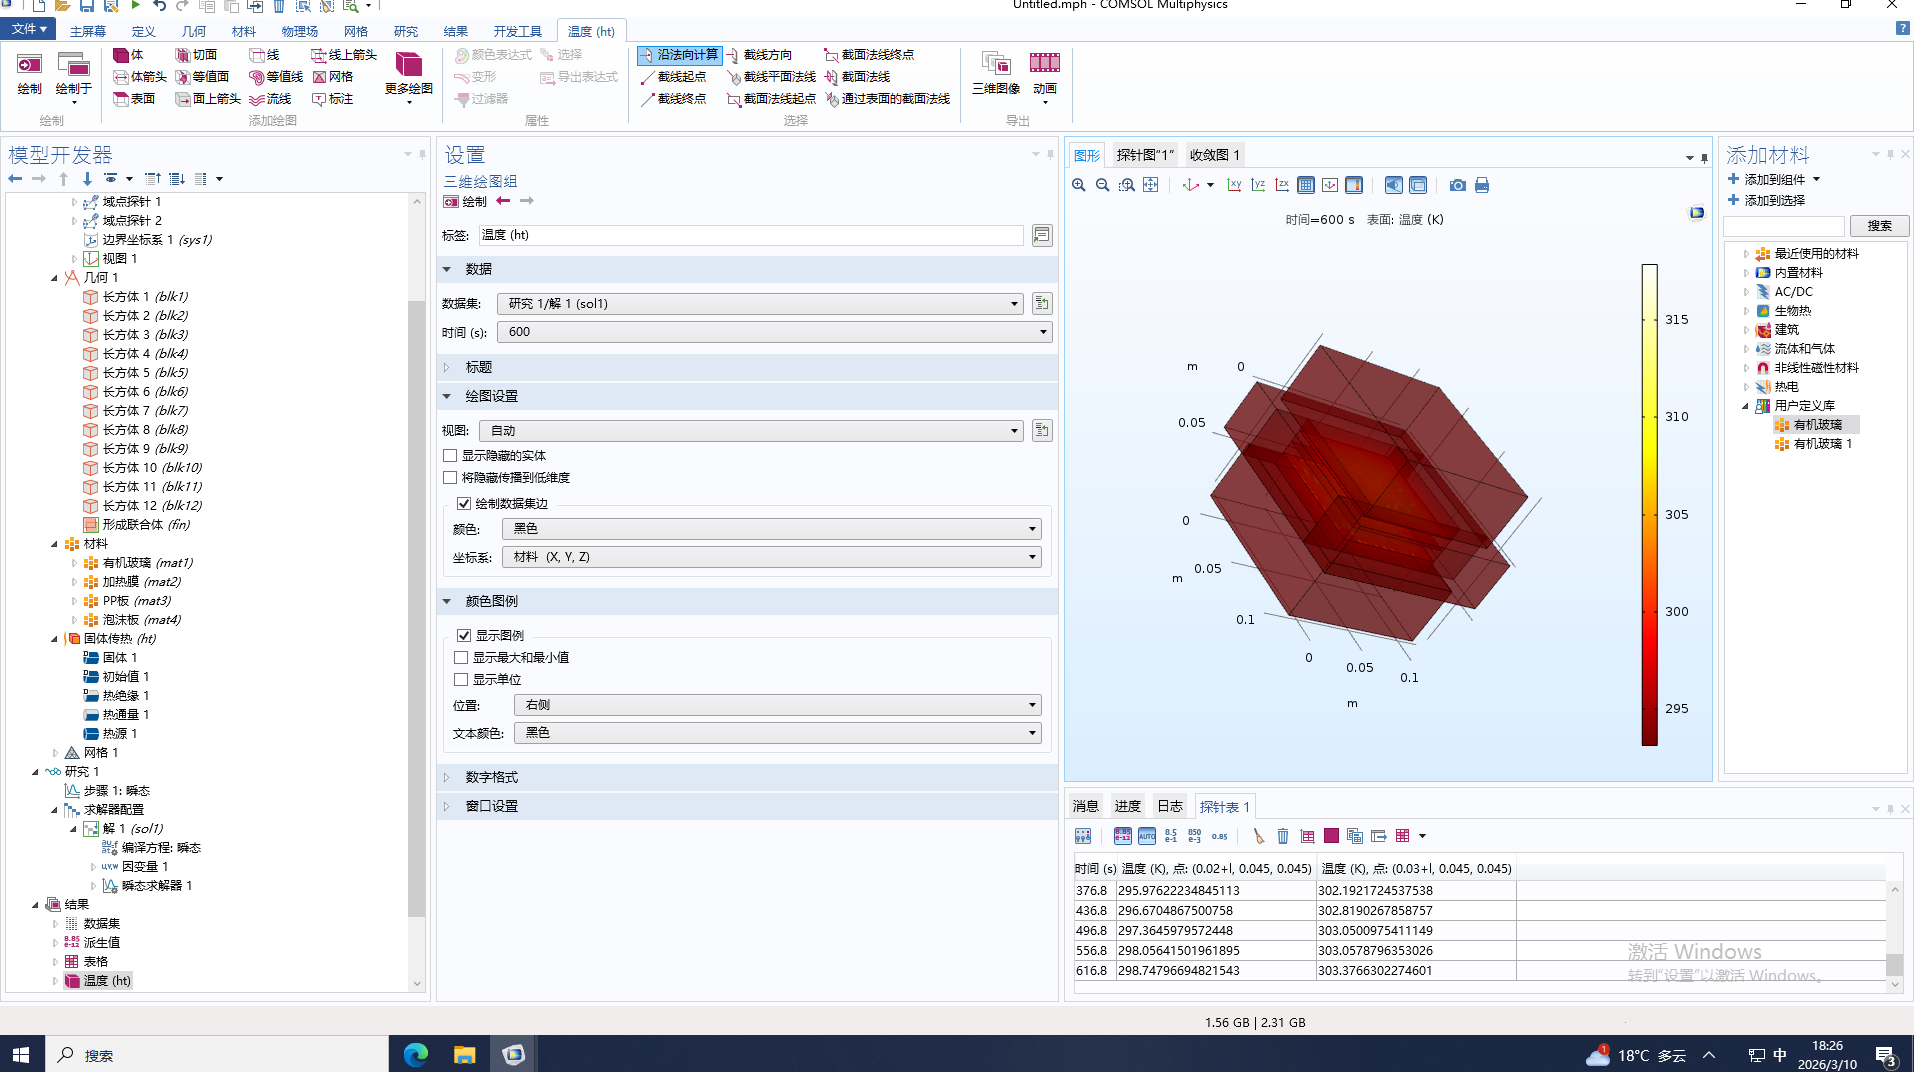
\includegraphics[width=0.95\columnwidth]{中心截面等温线.png}
  \caption{中心截面等温线分布（对称，与理论预期一致）}
  \label{fig:isothermal}
\end{figure}

由仿真数据，在$\Delta\tau=\SI{240}{\second}$（$t=\SI{994}{\second}\sim\SI{1234}{\second}$）区间：

\begin{itemize}
  \item 中心面升温速率：$\approx(305.11-302.78)/240\approx\SI{0.0097}{K/s}$；
  \item 加热面升温速率：$\approx(309.24-308.34)/240\approx\SI{0.0038}{K/s}$；
  \item 瞬时$\Delta T\approx\SI{4.13}{K}$，且仍在减小，系统尚未完全进入准稳态。
\end{itemize}

两探针升温速率差异表明该时段热量仍在向外传递，需更长时间（$\tau>\SI{1200}{s}$）才能达到准稳态。与实验值对比见表\,\ref{tab:compare}。

\begin{table}[H]
\centering
\caption{模拟（二）与实验值对比（有机玻璃16 V，近准稳态）}
\label{tab:compare}
\begin{tabularx}{\columnwidth}{lYY}
\toprule
 & $\Delta T$\,(\si{K}) & $\mathrm{d}T/\mathrm{d}\tau$\,(\si{K/s}) \\
\midrule
实验测量 & $\approx 4.6$ & $\approx 0.0067$ \\
模拟（二）（瞬时） & $\approx 4.13$ & $\approx 0.0097$ \\
\bottomrule
\end{tabularx}
\end{table}

当前仿真时段内两者量级一致，整体趋势与理论相符；延长仿真至完全准稳态后，预期$\Delta T$将进一步与实验值吻合。


%%%%%%%%%%%%%%%%%%%%%%%%%%%%%%%%%%%%%%%%%%%%%%%%%%%%%%%%%%%%
\section{思考题}

\begin{enumerate}
  \item \textbf{什么是第一类边条件（Dirichlet条件）、第二类边条件（Neumann条件）和第三类边条件（Robin条件），COMSOL能求解哪种边条件的问题？}\\[0.3em]
  第一类边条件（Dirichlet条件）直接规定边界上物理量的值，如$T|_\Gamma=T_0$；第二类边条件（Neumann条件）规定边界上物理量的法向导数，如$-\lambda\,\partial T/\partial n|_\Gamma=q$（热流密度）；第三类边条件（Robin条件）为前两类的线性组合，典型形式为$-\lambda\,\partial T/\partial n=h(T-T_\infty)$（对流换热）。COMSOL Multiphysics能够求解上述三种边条件的问题，并支持多物理场耦合情形下的混合边界条件设置。

  \item \textbf{选择四块板和两个加热膜（共六块）的情形下，为何膜的通电加热功率要乘以修正因子$A$？}\\[0.3em]
  实际实验中，加热膜面积有限，热量会从样品四周侧面散失，并非全部导入样品；加热膜自身也具有一定热容，会吸收部分热量。在仅含四块样品板和加热膜、侧面完全绝热的简化模型中，实际进入样品的有效热流密度小于理论计算值，因此需引入修正因子$A$（$A<1$）加以补偿，使仿真结果与实验测量值吻合。当模型中加入PP阻热层和泡沫隔热板后，热散失路径已被精确建模，此时取$A=1$即可获得与实验高度一致的仿真结果。
\end{enumerate}

%%%%%%%%%%%%%%%%%%%%%%%%%%%%%%%%%%%%%%%%%%%%%%%%%%%%%%%%%%%%
\clearpage
\onecolumn
\section*{参考文献}

\begin{enumerate}[label={[\arabic*]}]
  \item Heindlhofer K. Quenching: A Mathematical Study of Various Hypotheses on Rapid Cooling[J]. \textit{Physical Review}, 1922, 20: 221--242.
  \item Roznowski T. Temperature in Semi-infinite and Finite Cylinder with Moving Heating over the Lateral Surface[J]. \textit{Rozprawy Inzynierskie}, 1986, 34(1--2): 15--33.
  \item Ramakrishna K, Cohen I M, Ayyaswamy P S. Temperature Response of a Heated Cylinder Subject to Side Cooling: Asymptotic and Numerical Solutions[J]. \textit{ASME Heat Transfer Division (HTD)}, 1988, 104: 29--37.
  \item Jilani G, Jayaraj S, Ahmad M A. Conjugate Forced Convection-conduction Heat Transfer Analysis of a Heat Generating Vertical Cylinder[J]. \textit{International Journal of Heat and Mass Transfer}, 2002, 45(2): 331--341.
  \item Fukuya M, Terasaki T, Hasegawa K, et al. Numerical Analysis Method of Temperature Distribution in Cylindrical Steel during Quenching Process[J]. \textit{Solid State Phenomena}, 2006, 118: 355--362.
  \item Cossali G E. Periodic Heat Conduction in a Solid Homogeneous Finite Cylinder[J]. \textit{International Journal of Thermal Sciences}, 2009, 48: 722--732.
  \item 林琼桂. 高维波动方程与热传导方程非齐次边界条件的一般处理[J]. 大学物理, 2016, 35(5): 1--4.
  \item 姚端正. 一种实现边界条件与方程均齐次化的方法[J]. 大学物理, 2013, 32(3): 53--58.
  \item 郭敦仁. 数学物理方法[M]. 北京: 人民教育出版社, 1978: 300--303, 324--326.
  \item 梁昆淼. 数学物理方法[M]. 2版. 北京: 高等教育出版社, 1996: 374--378.
  \item 王刚, 安琳. COMSOL Multiphysics工程实践与理论仿真：多物理场数值分析技术[M]. 北京: 电子工业出版社, 2012: 72--83.
\end{enumerate}

\clearpage

\section{教师签名页}
  \begin{figure}[htbp]
  \centering
  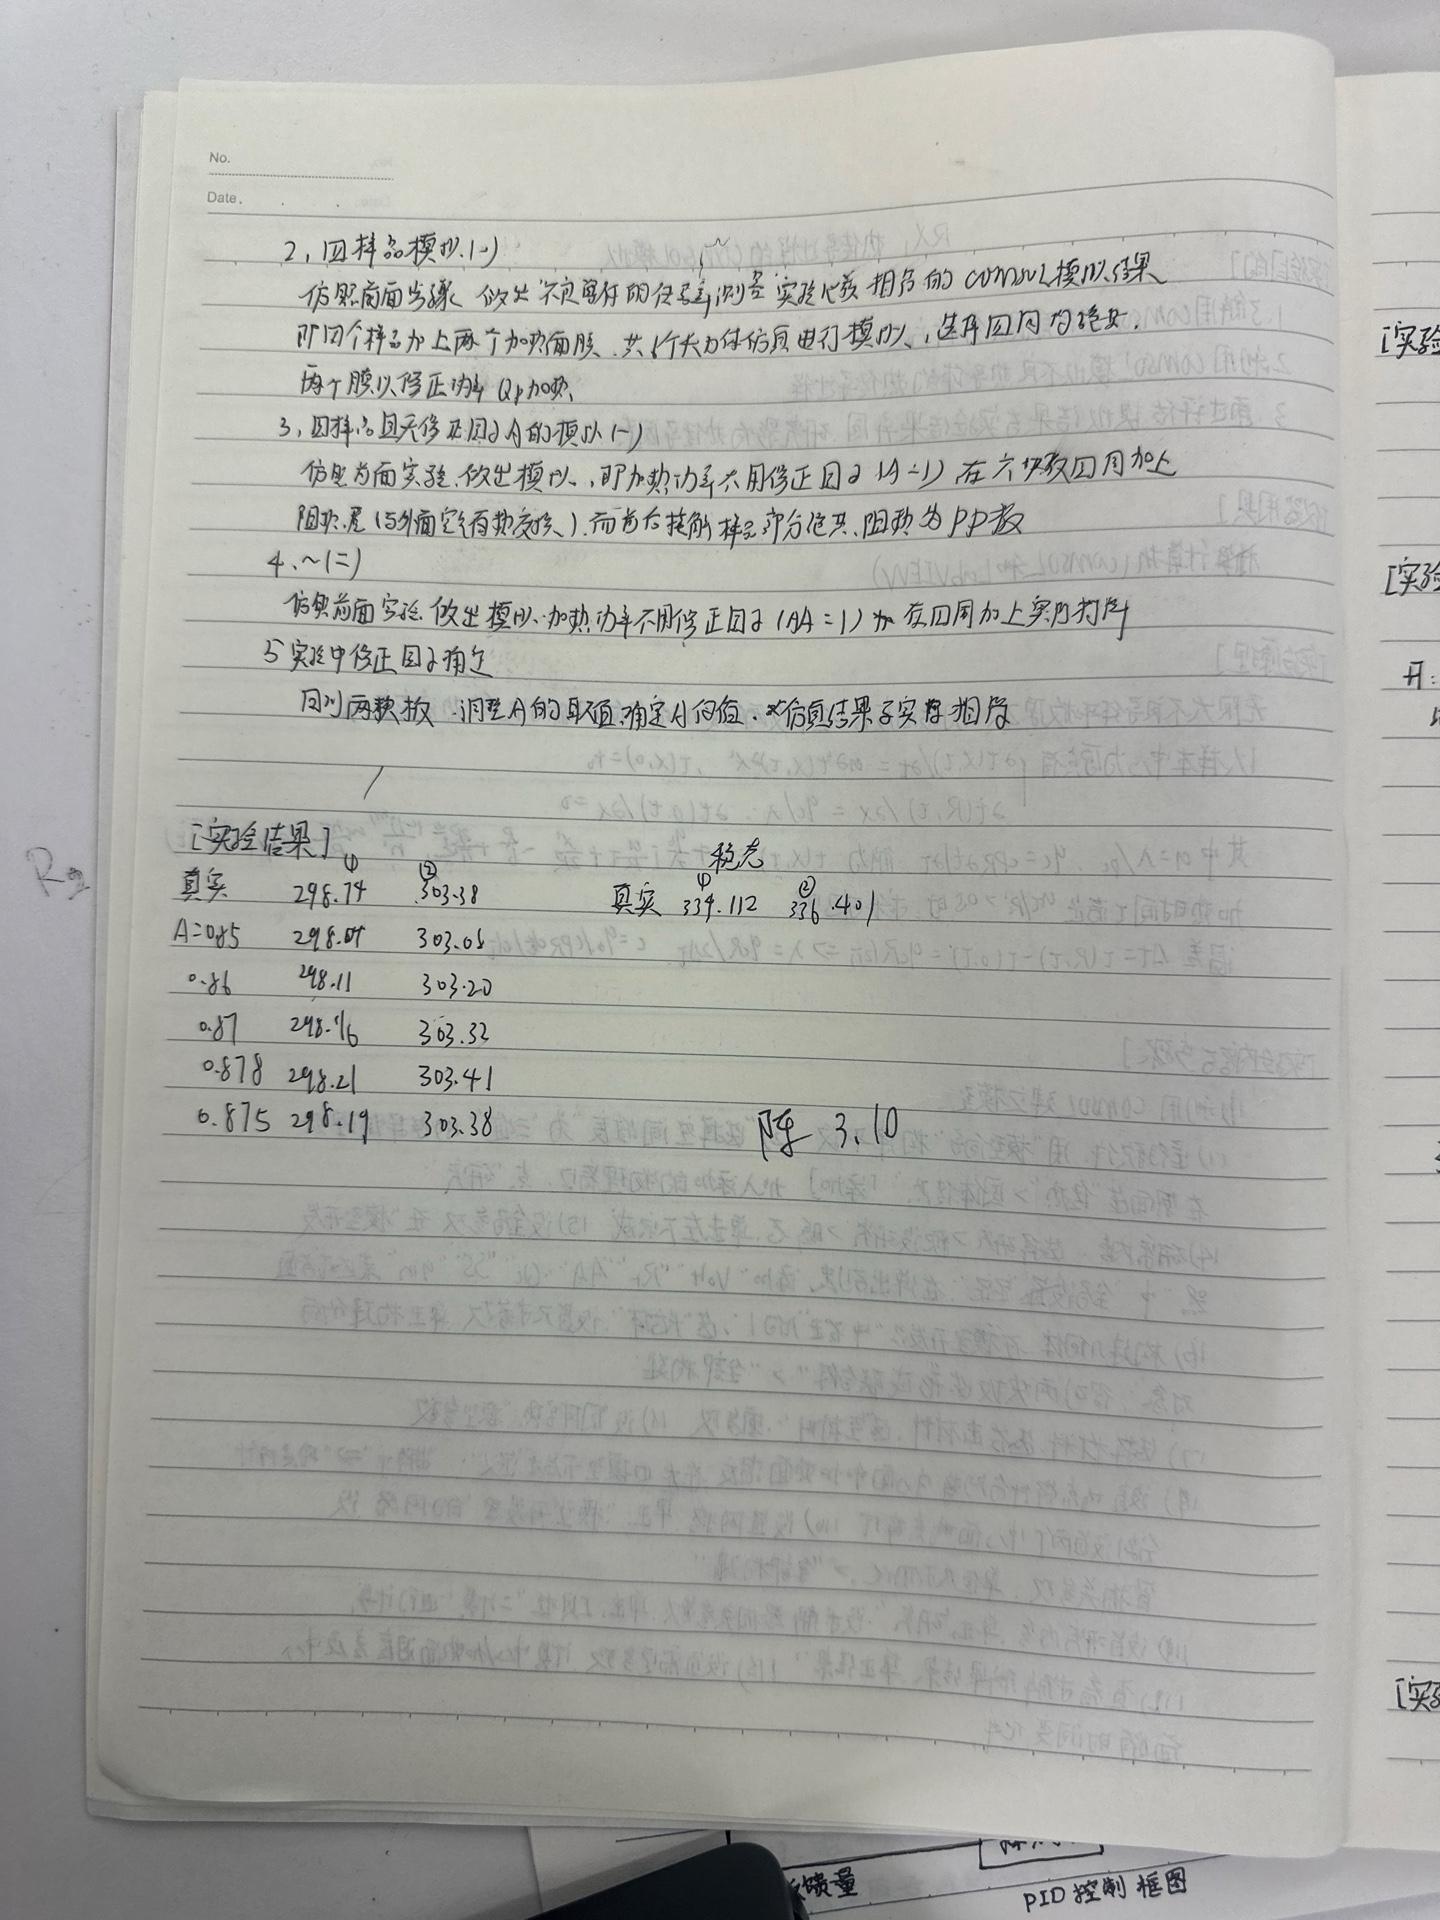
\includegraphics[scale=0.25]{教师签名页.png}
  \caption{教师签名页}
  \end{figure}

\end{document}
